%
% kruemmung2.tex
%
% (c) 2017 Prof Dr Andreas Müller, Hochschule Rapperswil
%
\documentclass[tikz]{standalone}
\usepackage{times}
\usepackage{txfonts}
\usepackage{pgfplots}
\usepackage{csvsimple}
\usetikzlibrary{arrows,intersections}
\begin{document}
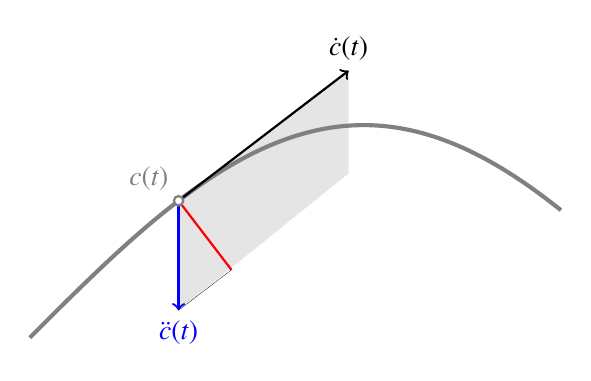
\begin{tikzpicture}[thick,scale=2.7]
\coordinate (O) at (0,0);

\def\deltax{0.5}
\def\vl{0.8}
\def\X{0.7}

%\draw[red,line width=0.7] (1.00000, 0.84147)--(1.82954,-0.69385);
%\draw[red,fill=blue]  (1.82954,-0.69385) circle[radius=0.04] {};
%\draw[red,fill=white] (1.82954,-0.69385) circle[radius=0.032] {};

\coordinate (A) at ({\X},{sin(180 * \X / 3.14159)});
\coordinate (B) at ({\X + \vl},{sin(180 * \X / 3.14159) + \vl * cos(180 * \X / 3.14159)});
\coordinate (C) at ({\X},{(1-\vl)*sin(180 * \X / 3.14159)});
\coordinate (D) at ({\X+\vl},{sin(180*\X/3.14159) + (1-\vl)*sin(180 * \X / 3.14159)});

\coordinate (G) at ({\X + cos(180 * \X / 3.14159)},{sin(180 * \X / 3.14159)-1});
\coordinate (H) at ({\X + \vl}, {(1-\vl) * sin(180 * \X / 3.14159) + \vl * cos(180 * \X / 3.14159)});

\coordinate (I) at (intersection of A--G and C--H);

\fill [fill=gray!20,line width=0] (A)--(B)--(D)--(C)--cycle;

\draw[gray,domain=0.0:2.5,line width=1.5,samples=100]
	plot (\x,{sin(180 * \x/3.14159)});

%\draw[gray,fill=red] ({\X},{sin(180 * \X / 3.14159)}) circle[radius=0.04] {};

\node at (A) [above left,gray] {$c(t)$};

%\draw[->] ({\X},{sin(180 * \X / 3.14159)})--({\X + \vl}, {sin(180 * \X / 3.14159) + \vl * cos(180 * \X / 3.14159)});
\draw[->] (A)--(B);

\node at (B) [above] {$\dot c(t)$};

\draw[->,blue] (A)--(C);

\draw[red] (A)--(I);
\draw[line width=0.1] (C)--(I);

\node[blue] at (C) [below] {$\ddot c(t)$};

\draw[gray,fill=white] ({\X},{sin(180 * \X / 3.14159)}) circle[radius=0.022] {};

\end{tikzpicture}
\end{document}
